\documentclass[titlepage,a4paper]{jsarticle}
\usepackage{../../../sty/import}% 各種パッケージインポート
\usepackage{../../../sty/title}% タイトルページの変更

%% タイトルページの変数
% レポートタイトル
\title{原子力材料と核燃料}
% 提出日
\expdate{\today}
% 科目名
\subject{原子力材料と核燃料}
% 分野
\class{情報経営システム工学分野}
% 学年
\grade{M1}
% 学籍番号
\mynumber{24336488}
% 記述者
\author{本間三暉}

\begin{document}
% titleページ作成
\maketitle

\section{$[110]$方向と$(110)$面}

結晶中の方向や面は，結晶軸を基準として指数で表される．
角括弧 $[uvw]$ は結晶中の方向を表し，丸括弧 $(hkl)$ は結晶面を表す．
したがって，$[110]$ と $(110)$ は同じ数字を用いているが，前者は方向，後者は面を意味する点で異なる．
以下では，立方晶の単位胞を考え，$[110]$ 方向と $(110)$ 面について述べる．

まず，$[110]$ 方向について考える．
結晶軸を $a$，$b$，$c$ とすると，$[110]$ 方向は $a$ 軸方向に1，$b$ 軸方向に1，$c$ 軸方向に0進む方向である．
すなわち，単位胞の原点を $(0,0,0)$ としたとき，$(1,1,0)$ に向かうベクトル方向である．
この方向は $c$ 軸方向の成分を持たないため，$ab$ 平面内の対角線方向として表される．
図\ref{fig:direction110}には，単位胞内における $[110]$ 方向を模式的に示す．
この図では，原点から $a$ 軸方向と $b$ 軸方向に等しく進む青い矢印として $[110]$ 方向を描くことができる．

\begin{figure}[H]
\centering
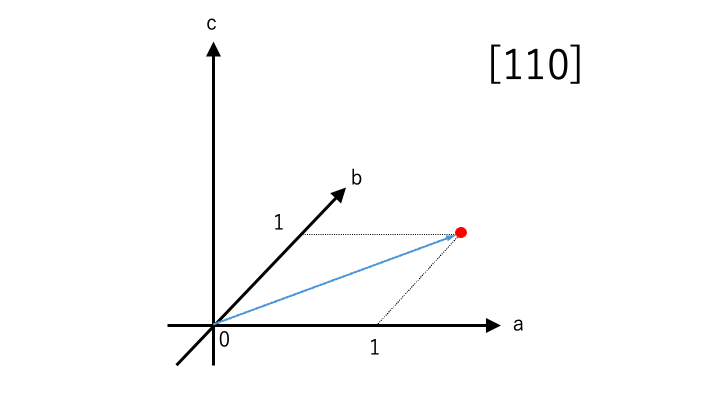
\includegraphics[width=0.55\linewidth]{img/direction110.png}
\caption{$[110]$方向}
\label{fig:direction110}
\end{figure}

次に，$(110)$ 面について考える．
ミラー指数 $(hkl)$ は，結晶面が各結晶軸をどこで切るかを表す指数である．
$(110)$ 面では，$h=1$，$k=1$，$l=0$ である．
したがって，この面は $a$ 軸を1の位置で切り，$b$ 軸も1の位置で切る．
一方，$l=0$ であるため，$c$ 軸とは交わらず，$c$ 軸に平行な面となる．
つまり，$(110)$ 面は，$ab$ 平面上では $(1,0,0)$ と $(0,1,0)$ を結ぶ線として見える．
三次元的には，その線を $c$ 軸方向に伸ばした面である．
$ab$ 平面上で切片だけを見ると，$a$ 軸方向と $b$ 軸方向にそれぞれ長さ $1$ の切片を持つため，座標軸と切片線によって直角二等辺三角形を考えることができる．
ただし，$(110)$ 面そのものは三角形ではなく，$c$ 軸方向に平行に伸びる結晶面である．
図\ref{fig:plane110}には，単位胞内における $(110)$ 面を示す．青い線で囲まれた領域が $(110)$ 面である．

\begin{figure}[H]
\centering
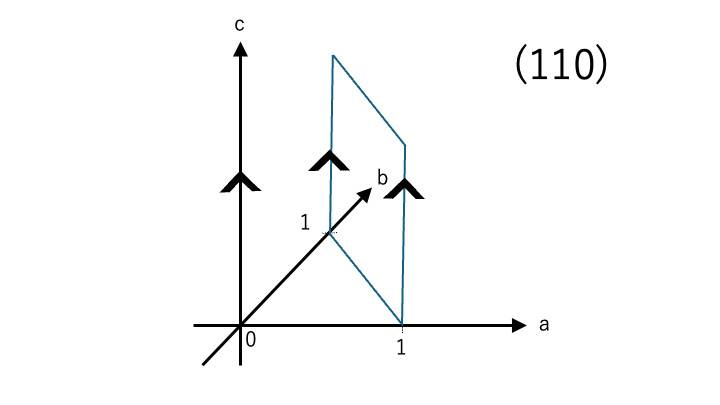
\includegraphics[width=0.55\linewidth]{img/plane110.png}
\caption{$(110)$面}
\label{fig:plane110}
\end{figure}

ここで重要なのは，$[110]$ 方向と $(110)$ 面を混同しないことである．
$[110]$ 方向は，原点から $(1,1,0)$ に向かう方向であり，$ab$ 平面内の対角線方向である．
一方，$(110)$ 面は，$a$ 軸と $b$ 軸をそれぞれ1で切り，$c$ 軸に平行な結晶面である．
また，立方晶では，$(hkl)$ 面に垂直な方向は $[hkl]$ 方向と対応する．
そのため，$(110)$ 面の法線方向は $[110]$ 方向となる．
したがって，$[110]$ 方向は $(110)$ 面の中に含まれる方向ではなく，立方晶においては $(110)$ 面に垂直な方向として理解する必要がある．

以上より，$[110]$ は結晶中の方向を表し，$a$ 軸方向と $b$ 軸方向に等しく進み，$c$ 軸方向成分を持たない方向である．
一方，$(110)$ は結晶中の面を表し，$a$ 軸と $b$ 軸を1で切り，$c$ 軸に平行な面である．
同じ ``110'' という指数を用いていても，角括弧と丸括弧の違いによって，方向と面という異なる幾何学的対象を表している．

% 参考文献
\begin{thebibliography}{99}
\bibitem{原子力材料と核燃料 講義資料}原子力材料と核燃料 講義資料
\end{thebibliography}

\end{document}